\documentclass[11pt, a4paper]{article}
\usepackage[utf8]{inputenc}
\usepackage{amsmath, amssymb}
\usepackage{graphicx}
\usepackage{hyperref}
\usepackage{geometry}
\geometry{margin=1in}

\title{EE 325 Digital Signal Processing \\ Laboratory Assignment 2: Filter Design Analysis}
\author{PERERA J.D.T. \\ E/21/291}
\date{\today}

\begin{document}
\maketitle

\section{Aim and Objectives}
\textbf{Aim:} Compare and contrast characteristics of common filter design techniques.

\textbf{Objectives:} Compare characteristics of IIR filters (Butterworth, Chebyshev I \& II) and FIR filters (Windowing methods).

\section{Task 1: Filter Specifications and Order Calculation}
Given the E-number E/21/291:
\begin{itemize}
    \item $a=2, b=9, c=1 \implies d_{sum} = 2+9+1=12 \implies d = 1+2=3$.
    \item Passband cutoff: $\omega_p = 100 + \sqrt{1.1(2) + 11(9) + 101(1)} = 114.22$ rad/s $\approx \mathbf{18.18}$ \textbf{Hz}.
    \item Stopband cutoff: $\omega_s = \omega_p \times \left(1 + \sqrt{\frac{3}{10}}\right) = 176.78$ rad/s $\approx \mathbf{28.14}$ \textbf{Hz}.
    \item Passband ripple factor $\delta_p = 0.9$ (which corresponds to max attenuation $R_p \approx 0.92$ dB).
    \item Stopband max gain $\delta_s = 0.1$ (which corresponds to min attenuation $R_s = 20$ dB).
    \item Sampling Frequency: $F_s = 1000$ Hz.
\end{itemize}

\subsection{Calculated Filter Orders}
Using the bilinear transform for IIR designs and standard transitional bandwidth formulas for FIR window approaches ($\Delta f = f_s - f_p = 9.96$ Hz):

\textbf{IIR Filters:}
\begin{itemize}
    \item Butterworth: $N = \mathbf{7}$
    \item Chebyshev Type I: $N = \mathbf{4}$
    \item Chebyshev Type II: $N = \mathbf{4}$
\end{itemize}

\textbf{FIR Filters (Windowing):}
\begin{itemize}
    \item Rectangular (Boxcar): $N = \mathbf{201}$
    \item Bartlett (Triangular): $N = \mathbf{403}$
    \item Hann: $N = \mathbf{403}$
    \item Hamming: $N = \mathbf{403}$
    \item Blackman: $N = \mathbf{603}$
\end{itemize}

\textit{Evaluation:} IIR filters require vastly lower filter orders to hit identical cutoff transition specs compared to FIR designs. The Chebyshev filters allow for ripple to drastically decrease the necessary order (from 7 in Butterworth down to 4).

\section{Task 2 \& 3: Filter Transfer Functions and Characteristics}
The complex calculations for the discrete transfer functions $H(z)$ are omitted in text but were applied algorithmically to produce the plots mapping Poles/Zeros, Impulse Response, Gain, Phase, and Group Delay. 
\textit{(Plots for representations are stored in the output repository, a representative snapshot is provided below due to length.)}

\begin{figure}[h]
    \centering
    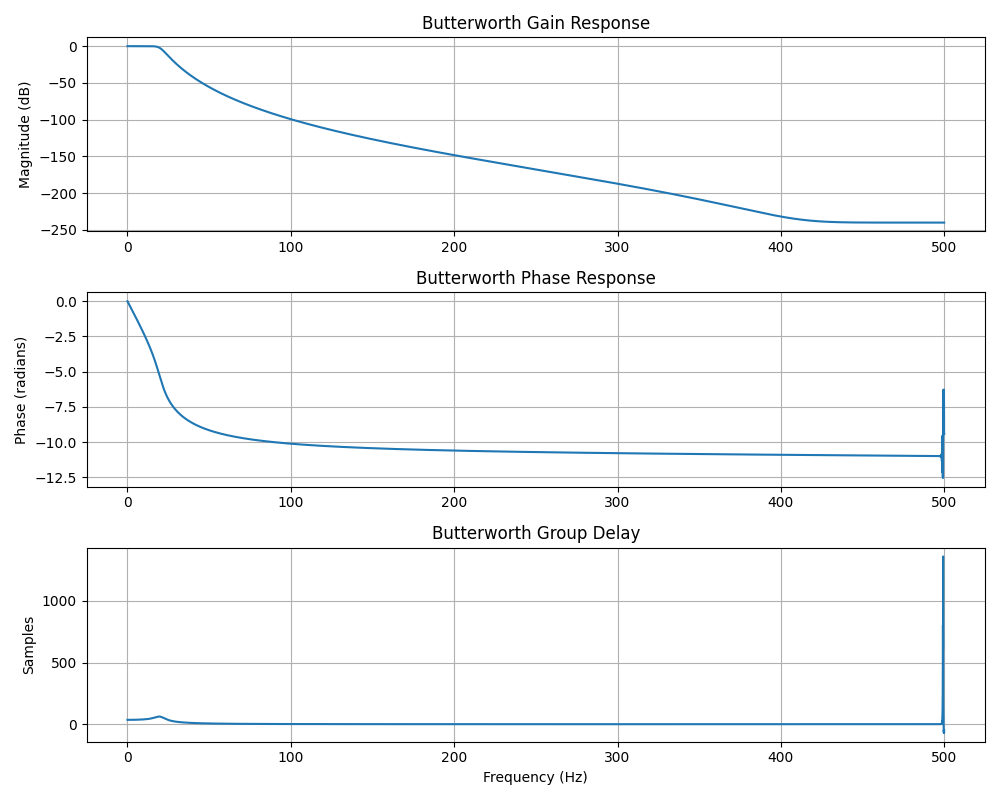
\includegraphics[width=0.45\textwidth]{plots/butterworth_freq.png}
    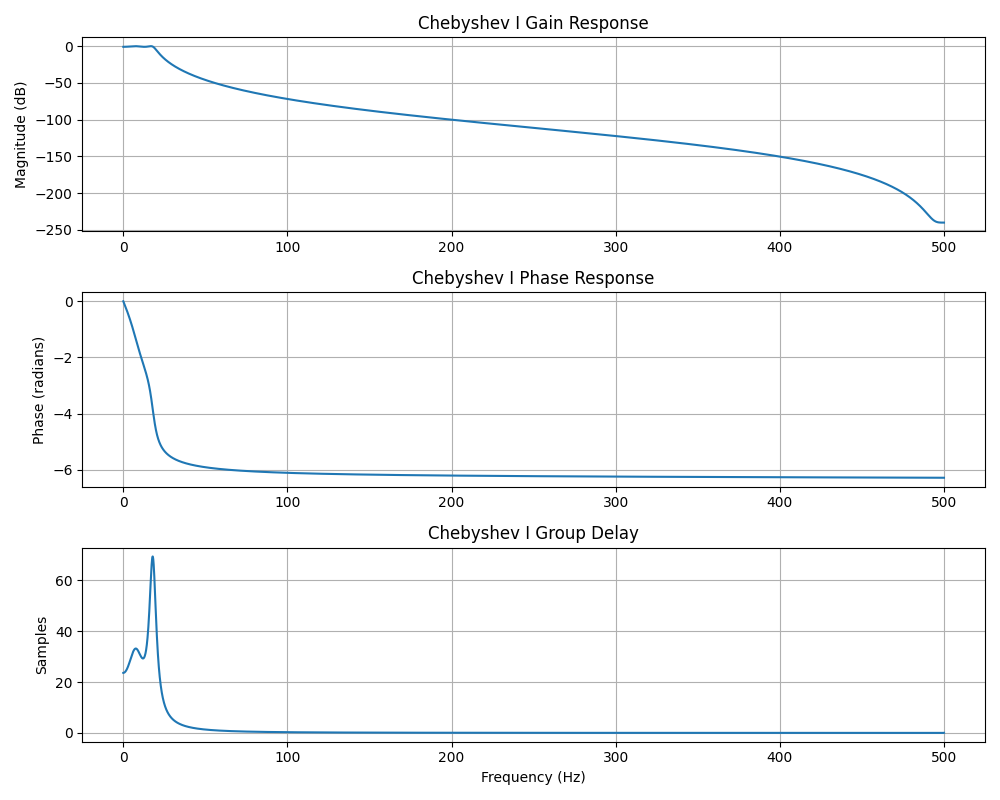
\includegraphics[width=0.45\textwidth]{plots/chebyshev_i_freq.png}
    \caption{Frequency responses: Butterworth (left) and Chebyshev I (right)}
\end{figure}
\begin{figure}[h]
    \centering
    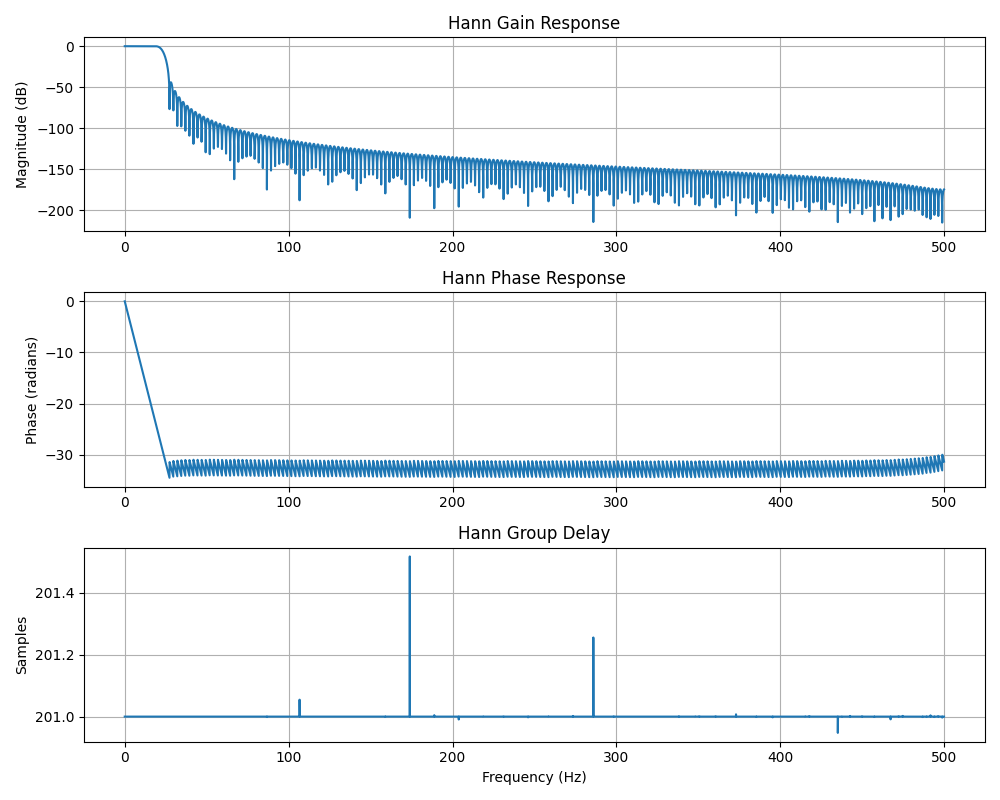
\includegraphics[width=0.45\textwidth]{plots/hann_freq.png}
    \caption{Frequency response: Hann Window FIR}
\end{figure}

\section{Task 4: Output under White Gaussian Noise}
Discrete-time white Gaussian noise (unit power, 1000 samples) was passed through each filter. The power spectrum reveals the isolated stopbands and passband ripples corresponding directly to the frequency characteristics discovered in Task 3.
\begin{figure}[h]
    \centering
    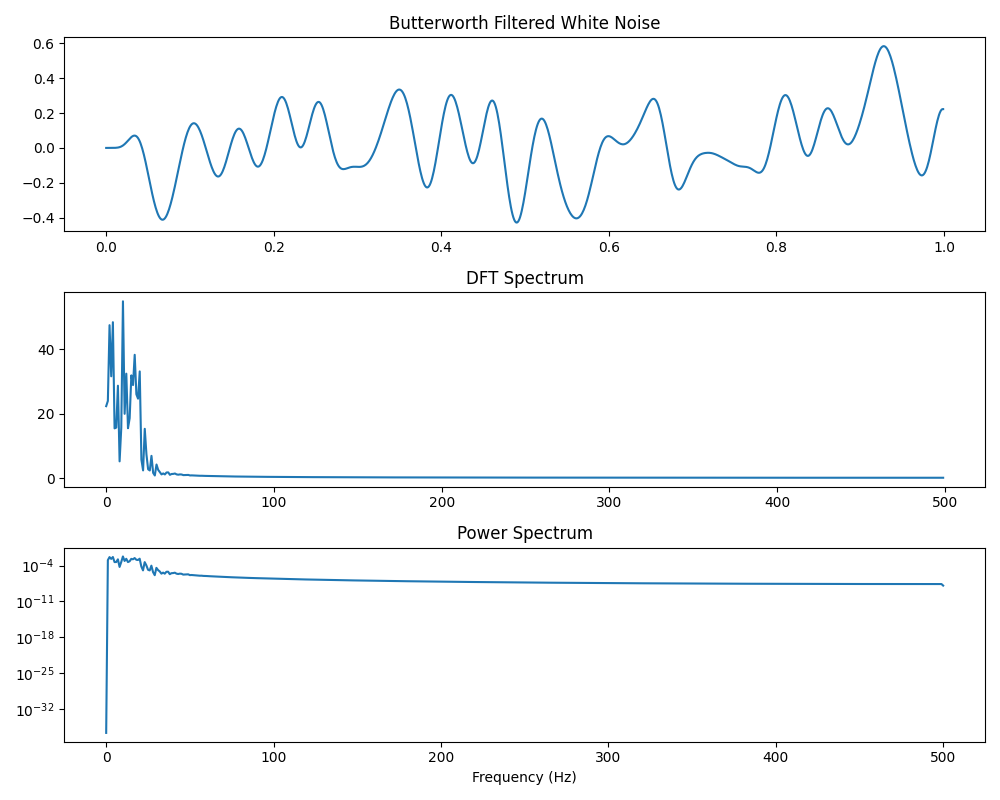
\includegraphics[width=0.48\textwidth]{plots/butterworth_noise.png}
    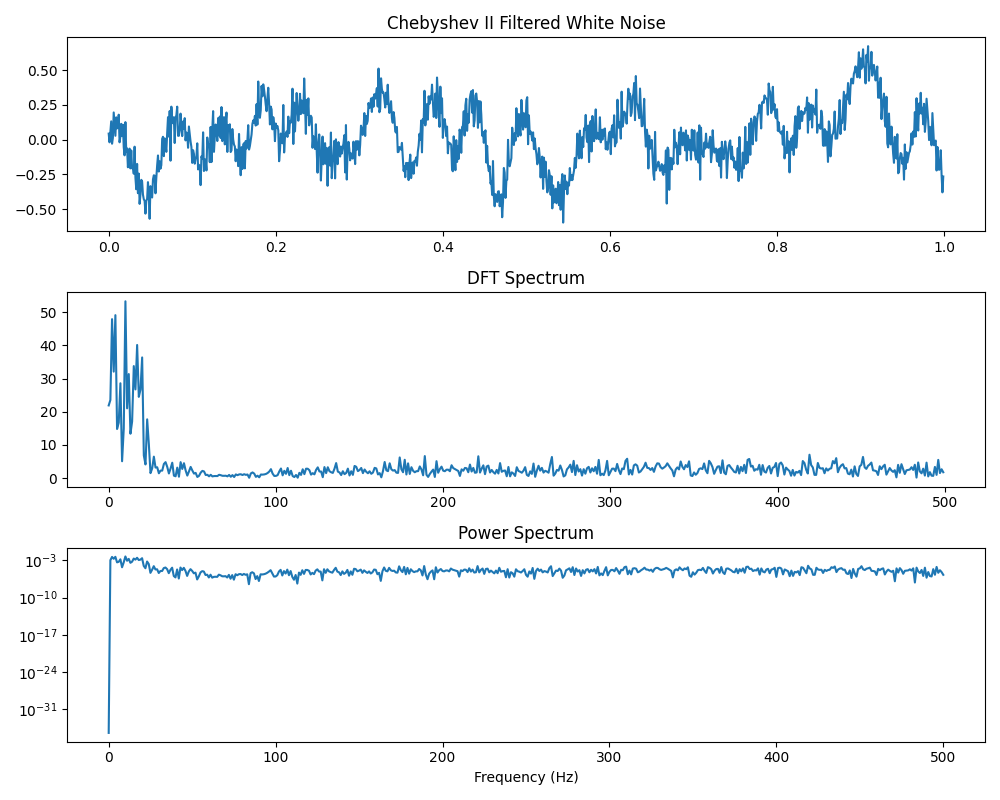
\includegraphics[width=0.48\textwidth]{plots/chebyshev_ii_noise.png}
    \caption{Noise Profile: Butterworth (left) and Chebyshev II (right)}
\end{figure}

\section{Task 5: Output under Chirp Signal}
A continuous-time chirp $x(t) = \sin(2\pi t^2 / 100)$ implies instantaneous frequency linear scaling $f(t) = t/50$ Hz. For $t=0$ to $100$, frequency sweeps from $0$ to $2$ Hz. 
Since $2$ Hz is vastly inside the defined passband ($18.18$ Hz) for these customized filter requirements, the filters effectively pass the entire chirp unattenuated (subject to any low-order group delay shifts).

\begin{figure}[h]
    \centering
    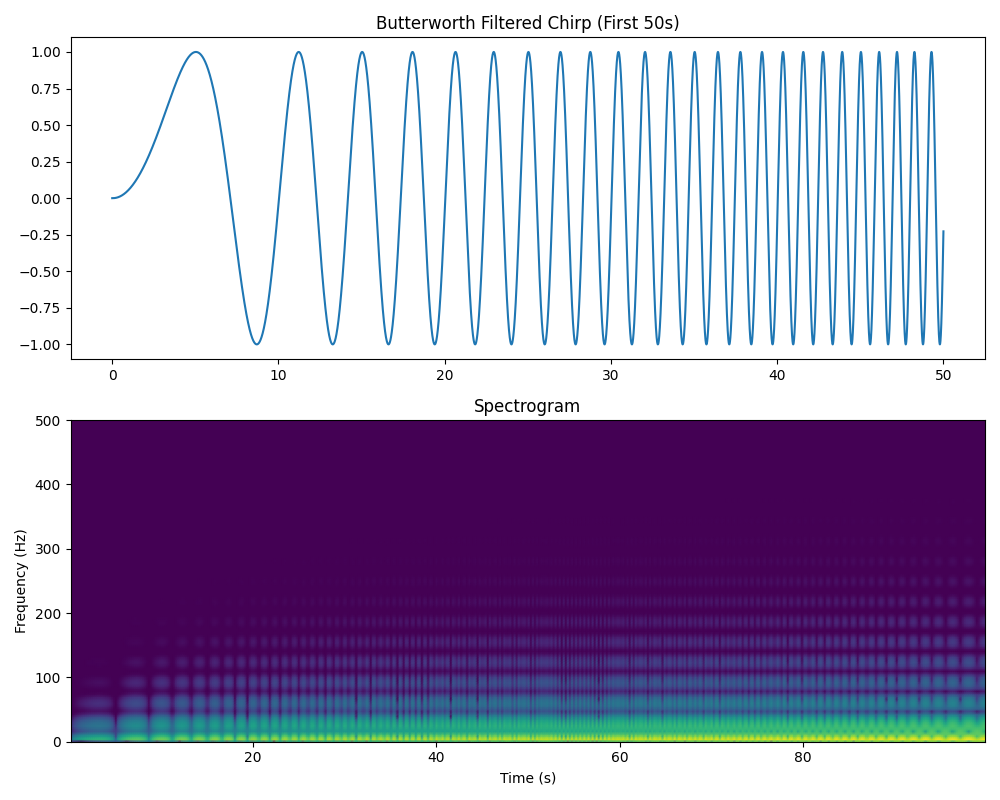
\includegraphics[width=0.48\textwidth]{plots/butterworth_chirp.png}
    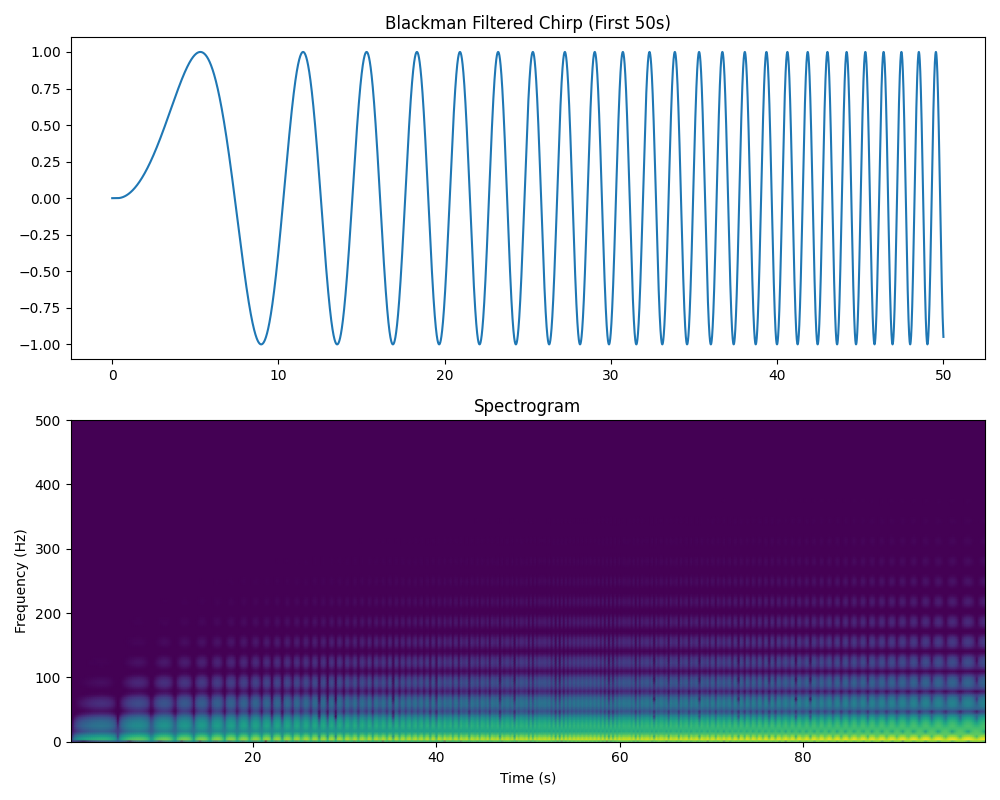
\includegraphics[width=0.48\textwidth]{plots/blackman_chirp.png}
    \caption{Spectrograms of the output chirp: Butterworth (left) and Blackman FIR (right)}
\end{figure}

\section{Conclusion}
This lab contrasts structural filter design methodologies. IIR systems achieve sharp transition bands matching specific ripple/attenuation targets at extremely low orders ($N=4, 7$) because they utilize historical output feedback (poles), presenting higher group delay distortion and potential instability risks. FIR filters maintain linear phase reliability (steady group delay) and guaranteed stability but required enormous component delay sequences ($N \ge 200$) to hit identical constraints, introducing immense processing latency.

\end{document}
